\documentclass[a4paper,11pt]{article}
\usepackage[utf8]{inputenc}
\usepackage[T1]{fontenc}
\usepackage{amsmath}
\usepackage{mathtools}
\usepackage{amsfonts}
\usepackage{amssymb}
\usepackage{graphicx}
\usepackage{multicol}
\usepackage{array}
\usepackage{float}
\usepackage{epstopdf}
\usepackage{caption}
\usepackage{subcaption}
\usepackage{gensymb}
\usepackage[bottom]{footmisc}
\usepackage{appendix}
\usepackage{pdfpages}
\usepackage{todonotes}
\usepackage{mathpazo}
\usepackage{titleps}
\usepackage{color}
\usepackage{xcolor}
\usepackage{colortbl}
\usepackage{siunitx}
\usepackage{pdflscape}
\usepackage{cancel}

\usepackage[skins]{tcolorbox}
\usepackage{sectsty}
\usepackage[arrowmos]{circuitikz}
\usepackage{pgfplots}
\usepackage{blindtext}
\usepackage[inner=2cm,outer=2cm,top=2.5cm,bottom=2.5cm]{geometry}
\usepackage{todonotes}
\usepackage{hyperref}
\usepackage{url}
\usepackage{adjustbox}
\usepackage{tabularx}
\usepackage{booktabs}
\usepackage{fancybox}
\usepackage[tikz]{bclogo}



%For code insertion
%listing
\usepackage{listings}
\usepackage{xcolor}
\definecolor{codegreen}{rgb}{0,0.6,0}
\definecolor{codegray}{rgb}{0.5,0.5,0.5}
\definecolor{codepurple}{rgb}{0.58,0,0.82}
\definecolor{backcolour}{rgb}{0.98,0.98,0.98}
\lstdefinestyle{mystyle}{
    backgroundcolor=\color{backcolour},
    commentstyle=\color{codegreen},
    keywordstyle=\color{blue},
    numberstyle=\tiny\color{codegray},
    stringstyle=\color{codepurple},
    basicstyle=\ttfamily\footnotesize,
    breakatwhitespace=false,
    breaklines=true,
    captionpos=b,
    keepspaces=true,
    numbers=left,
    numbersep=5pt,
    showspaces=false,
    showstringspaces=false,
    showtabs=false,
    tabsize=2
}
\lstset{style=mystyle}



\graphicspath{{figures/}}
\sectionfont{\large}
\subsectionfont{\normalsize}


\newpagestyle{main}{
	\sethead[LELEC2103][][]{LELEC2103}{}{}
	\headrule
    \setfoot[][\thepage][]{}{\thepage}{}
}

\newcommand{\horrule}[1]{\rule{\linewidth}{#1}} % Create horizontal rule command with 1 argument of height

%%%%%%%%%%%%%%%%%%%%%%%%%%%%%%%%%%%%%%%%%%%%%%%%%%%%%%%%%%%%%%%%%%%%%%%%%%%%

\begin{document}
\renewcommand{\figurename}{Fig.}

\renewcommand{\thepage}{\arabic{page}}
\setcounter{page}{1}
\pagestyle{main}
\newpage \clearpage

\begin{center}
\begin{LARGE}
LELEC2103: Optimization
\end{LARGE}
\vspace{0.3cm}
%\textit{TA 1, TA 2}
\end{center}

\section{Signal processing}
The space for improvement in the signal processing parts is very large.
Actually, you can consider any possible function that maps an audio sequence to an integer giving the predicted class. The only contextual constraint is that you must send somehow the acquired information wirelessly from the transmitter to the receiver. Then you also have to take into account the physical constraints imposed by your devices in terms of sampling, processing, memory, data rate and energy consumption. The priority when optimizing a working project is to identify the bottlenecks, i.e. the parts that are the most limiting the performances. Think about it before spending 3 weeks on something which would give negligible improvements at the end. To organize your reasoning, you can decompose the signal processing (without the authentication and packet creation aspects) in three main steps:

%%%%%%%%%%%%%%%%%%%%%%%%%%%%%%%%%%%%%%%%
\subsection{Feature vector shaping}
%%%%%%%%%%%%%%%%%%%%%%%%%%%%%%%%%%%%%%%%

\begin{figure}[H]
    \centering
    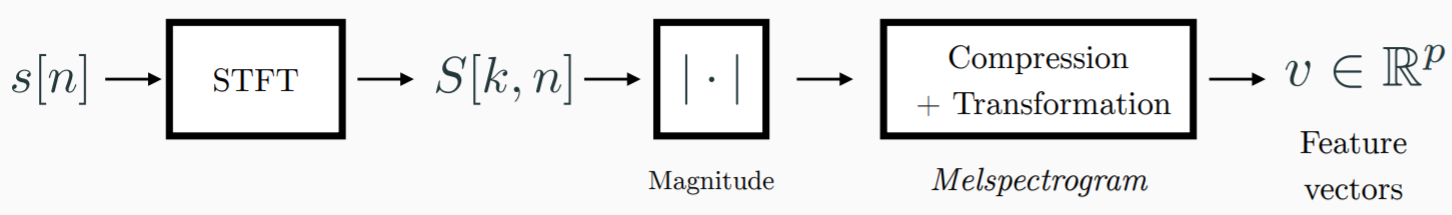
\includegraphics[width=14cm]{figs/scheme.PNG}
    \caption{Computation chain from temporal audio signal to feature vector.}
    \label{fig: fv}
\end{figure}
During the first semester, we provided you with a time-frequency representation that was compressed using the Hz$\rightarrow$mel transformation, as depicted in Figure \ref{fig: fv}. This choice is interesting because it yields intuitive observations and results for a human. To optimize this step, you can consider another block scheme. You could for instance choose another way of compressing the information than using Mels. Or you could keep a pure temporal representation and compress it another way.
However, this is not compulsory and we argue the current scheme in Figure \ref{fig: fv} is already efficient. \\
What can be done is to keep this scheme and play with its parameters. You can vary the window size and shape for the STFT. You can vary the number of mels. And mainly, these computations are all made in C code in a fixed-point representation. We voluntarily wrote non optimal code. \\
Finally, a way to save energy on your device is to avoid computing feature vectors when you think the currently acquired sound does not contain anything important. A first approach we can think of is an energy threshold, where we decide not to compute the feature vector if the sound is not loud enough.

To synthesize, some options are:
\begin{itemize}
    \item Change the feature vector computation scheme.
    \item Optimize this scheme by tuning its parameters and improving the
    fixed-point implementation.
    \item Imagine criteria for starting the computation of the feature vector.
\end{itemize}
%
%%%%%%%%%%%%%%%%%%%%%%%%%%%%%%%%%%%%%%%%
\subsection{Classification}
%%%%%%%%%%%%%%%%%%%%%%%%%%%%%%%%%%%%%%%%

\begin{figure}[H]
    \centering
    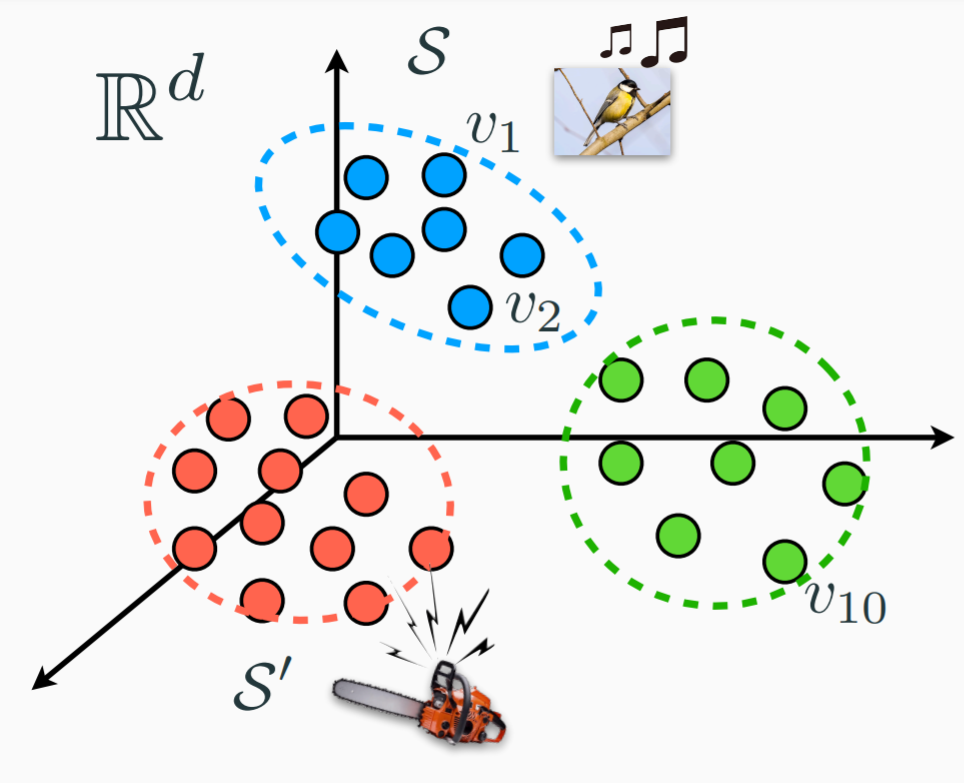
\includegraphics[width=8cm]{figs/classification.PNG}
    \caption{Classification principle.}
    \label{fig: classification}
\end{figure}
Once the feature vector computation process is fixed, the information contained in this feature vector has to be exploited at the receiver side for the classification, as shown in Figure \ref{fig: classification}. During the first semester, we already let you the possibility to play with different simple classifiers. The choice of the classifier is crucial and we advise you to test even more sophisticated ones to boost your perfomances. But remember to avoid overfitting! \\
You could consider the possibility to have a confidence metric on your predictions (remember that most classifiers provide first a probability of correct classification before to make a decision). This can be accompanied by a way to strenghten this confidence with the increasing amount of information provided by new features vectors. \\
Until now, you are classifying no matter what. There are situations where it is preferable not to output a prediction (i) the energy of the acquired sound is too low and you don't want to compute the feature vector on it (ii) your classifier outputs a probability vector balanced and no class is really highlighted. You are encouraged to manage these situations for the end of this project.


To synthesize, some options are:
\begin{itemize}
    \item Change the classifier.
    \item Add a confidence metric and exploit time to increase this confidence.
    \item Consider a threshold to output no class.
\end{itemize}

%%%%%%%%%%%%%%%%%%%%%%%%%%%%%%%%%%%%%%%%
\subsection{Training data}
%%%%%%%%%%%%%%%%%%%%%%%%%%%%%%%%%%%%%%%%

The way you train your classification model in this project is by using labelled (or training) data. This data is as important as the classifier choice. During the first semester, you trained your model with clean audio samples from the ESC-50 dataset, and discovered the possibility to augment this data by adding some transformations aiming to mimick real life perturbations. Now you master your devices and acquisition procedures, a better option is to create training data using your device. It implicitely takes the acquisition non idealities into account, and gives you the possibility to truly augment the data increasining the distance between the sound source and microphone, or adding background sound by yourself. \\
\\
Don't hesitate to discuss all your ideas with the TA's!

\newpage
\section{Crypto - How to perform a side-channel attack}
One of the proposed activities for this semester is about side-channel attacks. We propose you to evaluate the security of the cryptographic operations in your embedded sensor node against the power analysis side-channel attack.
For this purpose, you will use a methodology commonly used in side-channel security evaluation labs: take the role of an attacker and try to perform the best attack possible, that is, the one that uses the least amount of measurements.
To make the evaluation easier, evaluation labs often work on modified versions of the devices to analyze, which allows to performs the evaluation faster (e.g. cryptographic operations are run in a loop, and nothing else is done on the device).

In the following sections, we will show you how to obtain your first side-channel measurements, which we call traces. We then give you hints to mount your first attack, and finally give some practical informations.

\section{General idea}
The underlying idea of a side-channel attack is to exploit data dependent leakages emanating from the device under attack. More concretely, the CMOS circuit used on the MCU consumes power when the output of a logic gate flips from 0 to 1. Therefore, the current consumed by the MCU will be dependent on the data that is manipulated by the MCU. In \autoref{fig:leakage} you can see the current consumption of an MCU operation for different values.\\

\begin{figure}[h]
    \centering
    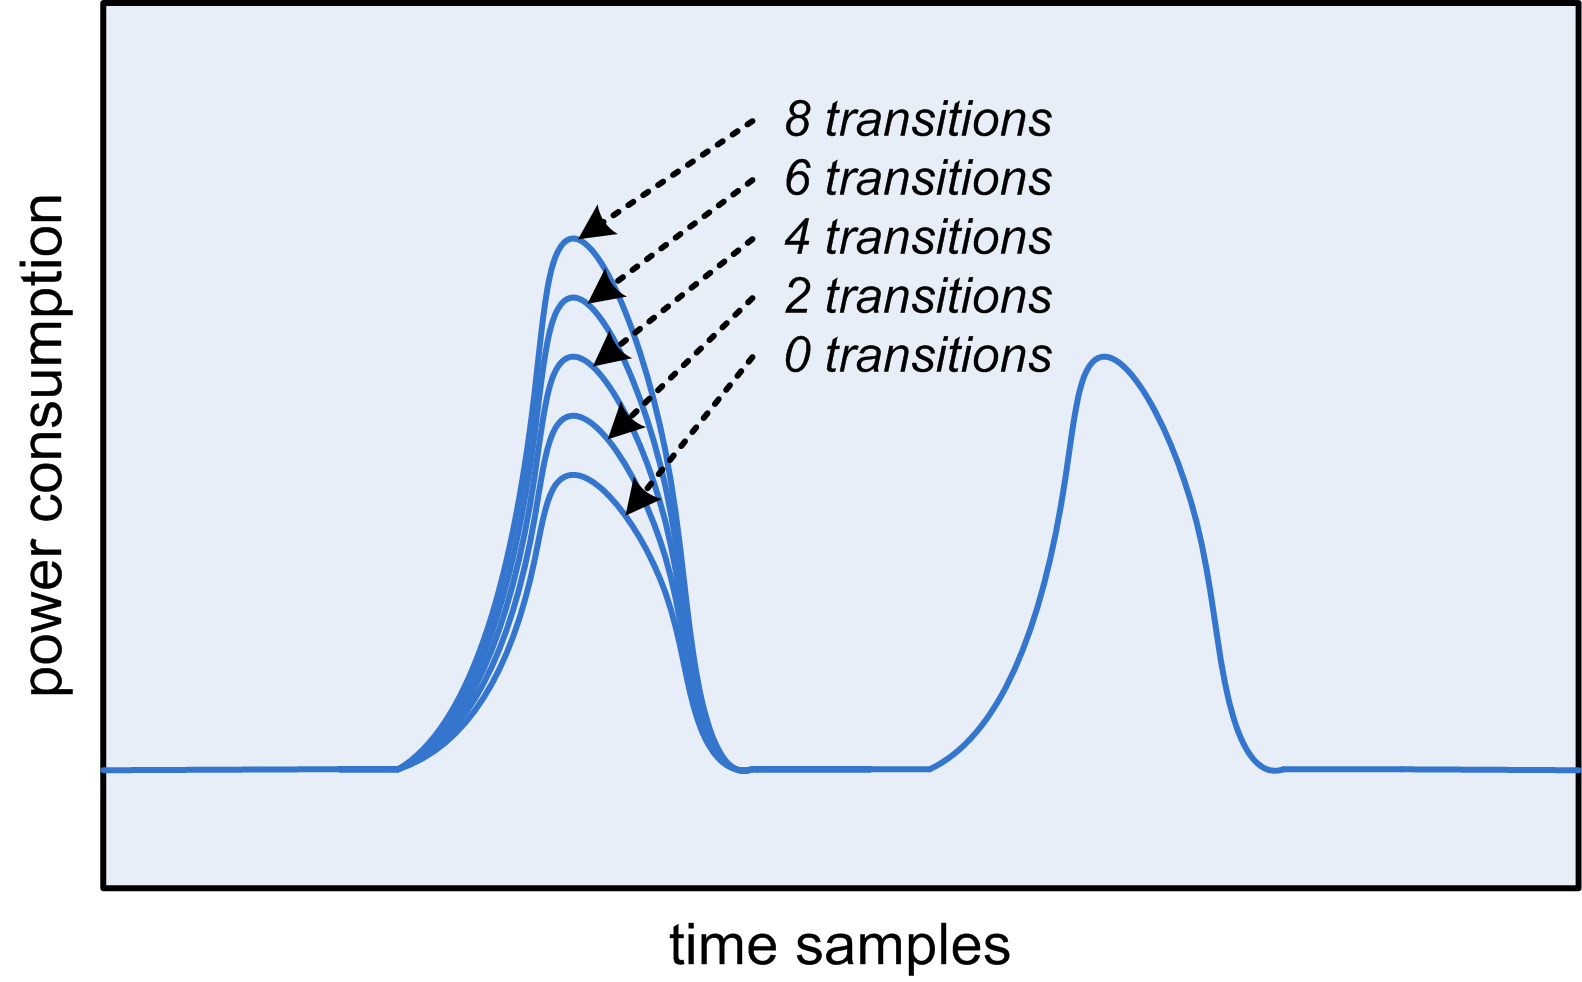
\includegraphics[width=0.5\linewidth]{figs/leakage.png}
    \caption{Power trace illustration for different values of manipulated data}
    \label{fig:leakage}
\end{figure}

To perform a side-channel attack, the attacker (in this case, you) collects measurements of the current consumption and then applies statistical tools to guess a secret value (usually the key for the encryption/authentication). We will show you in the next sections how to perform the current measurements. Then, for the statistical tools, we refer you to the LELEC2760 course material, more specifically, the 6th lecture and 3rd exercice session. All available at the following link : \url{https://perso.uclouvain.be/fstandae/LELEC2760_2022/}. \\

\section{How to prepare your setup}
Similarly to current measurements for the R7 report, you will have to place a shunt resistor on the power line of your MCU and measure the voltage drop on the resistor. You will be using a high performance Picoscope that you can borrow for your measurements.
\begin{bclogo}[couleur = gray!20, arrondi = 0.2, logo=\bcattention]{Picoscope vs ADALM2000}
The picoscope does not have a differential oscilloscope input. Therefore it is mandatory to connect the ground clip of the probe to the ground! Generally, the picoscope is a sensitive and expensive material. Please be cautious and respect at any time the input signal voltage ratings.
\end{bclogo}

\begin{bclogo}[couleur = gray!20, arrondi = 0.2, logo=\bcinfo]{Measurement setup differences from R7 report}
In the context of side-channel meausrements, we are not interested in the absolute value of consumed current, but in the small relative change between measurements. This allows the simplification of the setup in many ways:
\begin{itemize}
    \item Assuming that the 3.3V source connected to the resistor is stable enough, we can connect only one probe and avoid subtracting the result of 2 channels.
    \item The coupling of the oscilloscope can also be changed to AC, improving the vertical resolution of our measurements.
\end{itemize}
\end{bclogo}
When performing side-channel attacks, the attacker needs to synchronize the traces such that each time sample corresponds to the same operation on the MCU, independent of the measurement number. There exists algorithms to perform such alignment from the power traces themselves, but (as commonly used for in evaluation labs), we will skip this step and acquire aligned traces thanks to the use of an additional trigger signal. This trigger signal is a GPIO pin that is set to high just before the beginning of each AES encryption and is set to low after it finishes. This trigger signal will be used as the trigger of the oscilloscope. It is routed on the \textbf{rightmost} (closest to the PCB corner) pin of the \textbf{CTRLS} header on the audio acquisition PCB.

\section{How to acquire traces}
You will have to install a few packages first :
\begin{enumerate}
\item Follow \url{https://www.picotech.com/downloads/linux} to install the Picoscope libraries and software. Note that installing the software automatically installs libraries.
    \item Then install the following python packages: \texttt{numpy scipy matplotlib picosdk}.
\end{enumerate}

Next, read and understand the MCU code that is available on the integration git on the crypto\_DPA branch\footnote{\url{https://forge.uclouvain.be/lelec2102-2103/integration/-/tree/crypto_DPA}}. This code is slightly different from the full project as it only running the AES with per-dertermined plaintexts (again, this is an artificial setup which makes the attack easier to mount for evaluation purposes).

Use the \texttt{collect\_basic.py} acquisition script to collect the traces. You should press the blue button to start encryptions only when the Picoscope is ready. This and the following scripts are located in the \texttt{scripts/sca} folder. This scripts configures the picoscope, you may want to tune this configuration (although the one we give should be sufficient for your first attack).

In order to perform analysis over the traces, you should know the inputs of the AES that were used. To do so, use \texttt{gen\_inputs.py} that replicates the pseudo-random-generator (PRG) implemented on the MCU to derive the inputs (plaintexts) of the AES executions. Make sure that the seed of the PRG is the same on the MCU and in the script. (This PRNG is the reason why it is important that you start the execution of the AES on the MCU only after the picosope is ready to acquire traces: otherwise, the plaintexts generated by the script will not correspond to the acquired traces.)

The remaining file is \texttt{scascope.py} which provides an easy to use interface to the Picoscope library and is used by \texttt{collect\_basic.py}. Some configuration options of the picoscope can be set from here and not from \texttt{collect\_basic.py}.
During acquisition, you should connect the trigger signal as EXT (otherwise you would have to configure two acquisition channels, which wastes precious acquisition memory in the picoscope). You should also aim your signal to fill the vertical range of your scope without overflowing.

\begin{bclogo}[couleur = gray!20, arrondi = 0.2, logo=\bcinfo]{Usage of Picoscope software}
Altough we use scripts to acquire the traces, we advise you to use the Picoscope software to fine tune your setup parameters such as resistor value, vertical range, etc. You can also visualize the trigger signal (for this usage, put in on one of the channels) to learn the timing range you need to sample.

Try to visualize features in the signal: can you visually see patterns in the signal? Is there noise? You can also have a look at the signal in the frequency domain!
\end{bclogo}

\section{Advice for your first attack}
In addition to the classical oscilloscope parameters (vertical and horizontal range), you can play with other variables in this setting : the sampling rate, the vertical resolution. This Picoscope can also do resolution augmenting, that is, averaging multiple samples to obtain higher vertical resolution. As it has a 12 bit ADC, and a maximum sampling rate of 250MS/s, you can reduce the sampling rate for better resolution. We advise you to analyse this tradeoff. (But, for your first attack, the default configuration we gave should work.)

For your first attack, it is necessary to preprocess the traces with a bandpass filter to reduce the noise of unnecessary frequency domains. The \texttt{dpa.py} script contains such a basic filter. Feel free to improve it or remove it for advanced attacks.

As a first side-channel attack, you should aim for the basic \textit{single-bit differential power analysis (DPA)}. You should be able to recover the correct key bytes with 200k traces for the vast majority of the bytes. Then you should optimize your setup. To do so, you can either look at the physical setup, oscilloscope parameters, signal processing, statistical analysis.

The acquisition script can only record 100k traces in the current configuration (due to limited internal memory of the picoscope), but you can make two recordings of the execution (resetting the MCU in-between, but using the same key and PRNG seed), then average the corresponding traces to reduce the physical noise of your measurements (you may also do it with more than 2 recordings).

\section{Booking modalities}
The Picoscopes can be borrowed for at most one day -- they cannot leave the Maxwell building.
In order to book one, you should send an email to \url{gaetan.cassiers@uclouvain.be} \textbf{AND} \url{balazs.udvarhelyi@uclouvain.be}, if possible 2 days in advance. You can retrieve and deposit the Picoscopes at the Maxwell b.125 office.

Do not forget to record your traces in properly labelled and documented files such that you can run and improve the attacks offline, without the Picoscope.

\section{Contest rules}
You were given a MCU project for which you know the source code and can set the key, such that you are in total control of your setup.
During the contest, we will flash the MCU with a binary built from the exact same source code (at -O3 optimization level) but with two differences: the key will be new, and the delay between two AES executions might be modified.\footnote{%
    Maybe you won't be able to acquire 100k traces in a few seconds anymore\dots
}
Your goal will be to recover the secret key as fast as possible.
Finally, a few plaintext/ciphertext pairs will be given to you along with your flashed MCU (e.g., to test if your key guess is correct, or to perform more advanced attacks).


\end{document}
%%%%%%%%%%%%%%%%%%%%%%%%%%%%%%%%%%%%%%%%%%%%%%%%%%%%%%%%%%%%%%%%%%%%%%%%%%%%
